% VoiceNotion - Chapitre II: Planification et Conception UX
% Ce chapitre présente la planification du projet et la conception de l'expérience utilisateur

\chapter{PLANIFICATION ET CONCEPTION UX}

\section{Introduction}

Après avoir identifié les problématiques et défini le concept de VoiceNotion dans le chapitre précédent, nous nous concentrons maintenant sur la planification du projet et la conception de l'expérience utilisateur. Cette phase est cruciale pour transformer notre vision en un plan d'action concret et en une interface utilisateur intuitive qui répond aux besoins réels des utilisateurs.

La planification et la conception UX sont particulièrement importantes pour VoiceNotion en raison de son approche novatrice combinant commandes vocales et édition par blocs. L'interaction vocale, bien que naturelle pour la communication humaine, présente des défis uniques lorsqu'elle est appliquée au contrôle d'une interface numérique. Notre objectif est de créer une expérience fluide et intuitive qui tire pleinement parti des capacités vocales tout en offrant une interface visuelle cohérente et familière.

Ce chapitre détaille notre méthodologie de planification, notre approche de l'expérience utilisateur basée sur la recherche et l'empathie, ainsi que la conception technique du système d'information qui sous-tend l'application.

\section{Planification du projet}

\subsection{Méthodologie de planification}

Pour le développement de VoiceNotion, nous avons adopté une approche agile, plus précisément la méthodologie Scrum, complétée par des éléments de Design Thinking pour la conception UX. Cette combinaison nous permet d'itérer rapidement tout en gardant l'utilisateur au centre de notre processus de conception.

\subsubsection{Approche Agile Scrum}

L'approche Scrum a été choisie pour sa flexibilité et sa capacité à s'adapter aux changements inhérents au développement d'un produit innovant comme VoiceNotion. Nous avons organisé notre travail en sprints de deux semaines, chacun comportant les événements standards de Scrum:

\begin{itemize}
    \item \textbf{Sprint Planning:} Au début de chaque sprint, l'équipe sélectionne les tâches du Product Backlog à réaliser, en se basant sur leur priorité et la capacité de l'équipe.
    
    \item \textbf{Daily Stand-up:} Réunions quotidiennes de 15 minutes pour synchroniser les activités et identifier les obstacles.
    
    \item \textbf{Sprint Review:} À la fin de chaque sprint, l'équipe présente les fonctionnalités développées aux parties prenantes pour obtenir des retours.
    
    \item \textbf{Sprint Retrospective:} L'équipe analyse ce qui a bien fonctionné et ce qui peut être amélioré pour le prochain sprint.
\end{itemize}

Cette approche nous permet de livrer régulièrement des incréments de produit fonctionnels et d'ajuster notre direction en fonction des retours utilisateurs et des défis techniques rencontrés.

\subsubsection{Design Thinking pour l'UX}

En parallèle de Scrum, nous avons intégré le processus de Design Thinking pour la conception de l'expérience utilisateur, qui comprend cinq phases:

\begin{enumerate}
    \item \textbf{Empathie:} Comprendre profondément les besoins, les frustrations et les aspirations des utilisateurs potentiels à travers des entretiens et des observations.
    
    \item \textbf{Définition:} Synthétiser les connaissances acquises pour définir clairement les problèmes à résoudre.
    
    \item \textbf{Idéation:} Générer un large éventail d'idées et de solutions potentielles sans contraintes initiales.
    
    \item \textbf{Prototypage:} Créer des représentations tangibles des solutions les plus prometteuses.
    
    \item \textbf{Test:} Recueillir les retours des utilisateurs sur les prototypes pour affiner et améliorer les solutions.
\end{enumerate}

Cette approche centrée sur l'utilisateur est particulièrement pertinente pour VoiceNotion, où l'interaction vocale nécessite une compréhension fine des attentes et des comportements des utilisateurs.

\begin{figure}[H]
    \centering
    %\includegraphics[width=0.8\textwidth]{assets/docs/agile_design_thinking.png}
    \caption{Intégration de Scrum et Design Thinking dans notre méthodologie}
    \label{fig:agile_design_thinking}
\end{figure}

\subsection{Planification}

\subsubsection{Roadmap du projet}

La roadmap de VoiceNotion a été structurée en quatre phases principales, chacune comportant plusieurs sprints:

\begin{enumerate}
    \item \textbf{Phase de recherche et de conception (2 mois):}
    \begin{itemize}
        \item Recherche utilisateur et analyse concurrentielle
        \item Définition des personas et des scénarios d'utilisation
        \item Conception de l'architecture du système
        \item Wireframing et prototypage initial
    \end{itemize}
    
    \item \textbf{Phase de développement MVP (4 mois):}
    \begin{itemize}
        \item Mise en place de l'infrastructure technique
        \item Développement du backend et de l'API
        \item Implémentation de l'éditeur de notes par blocs (avec BlockNote.js)
        \item Intégration de la reconnaissance vocale de base
        \item Développement de l'interface utilisateur mobile (Expo/React Native)
    \end{itemize}
    
    \item \textbf{Phase d'amélioration et d'expansion (3 mois):}
    \begin{itemize}
        \item Optimisation des algorithmes de traitement du langage naturel
        \item Expansion des commandes vocales supportées
        \item Développement de l'interface web
        \item Implémentation des fonctionnalités de sous-pages et de hiérarchie de notes
    \end{itemize}
    
    \item \textbf{Phase de finalisation et de lancement (1 mois):}
    \begin{itemize}
        \item Tests utilisateurs approfondis
        \item Correction des bugs et optimisations finales
        \item Préparation du matériel marketing
        \item Lancement officiel de l'application
    \end{itemize}
\end{enumerate}

\subsubsection{Gestion des risques}

Nous avons identifié plusieurs risques potentiels pour le projet et élaboré des stratégies d'atténuation:

\begin{table}[H]
\centering
\begin{tabular}{|p{3cm}|p{5cm}|p{5cm}|}
\hline
\textbf{Risque} & \textbf{Impact potentiel} & \textbf{Stratégie d'atténuation} \\
\hline
Précision limitée de la reconnaissance vocale & Frustration utilisateur, abandon de l'application & Implémentation d'un mécanisme de correction, modes d'entrée alternatifs, tests extensifs avec différents accents \\
\hline
Complexité technique de l'intégration BlockNote & Retards de développement, problèmes de performance & Spike techniques précoces, exploration des alternatives, recrutement d'expertise spécifique \\
\hline
Expérience utilisateur non intuitive & Courbe d'apprentissage abrupte, faible adoption & Tests utilisateurs fréquents, approche itérative, tutoriels intégrés \\
\hline
Limites des API Gemini & Fonctionnalités restreintes, dépendance à un tiers & Plan de secours avec solutions alternatives, découplage de l'architecture \\
\hline
Problèmes de performance sur appareils mobiles & Lenteur, consommation excessive de batterie & Optimisation continue, tests sur différents appareils, métriques de performance \\
\hline
\end{tabular}
\caption{Tableau des risques et stratégies d'atténuation}
\label{tab:risk_management}
\end{table}

\section{Expérience d'utilisateur (UX)}

\subsection{Recherche}

La conception de VoiceNotion est fondée sur une recherche approfondie pour comprendre les besoins, les attentes et les points de friction des utilisateurs potentiels en matière de prise de notes.

\subsubsection{Méthodologie de recherche}

Notre recherche a combiné plusieurs approches:

\begin{itemize}
    \item \textbf{Entretiens qualitatifs:} Nous avons mené 15 entretiens approfondis avec des utilisateurs potentiels issus de nos groupes cibles (étudiants, professionnels, créateurs de contenu).
    
    \item \textbf{Analyse concurrentielle:} Étude détaillée des applications existantes (Notion, Evernote, OneNote, Google Keep) pour identifier les forces, les faiblesses et les opportunités d'innovation.
    
    \item \textbf{Sondage en ligne:} Un questionnaire distribué à 150 participants pour quantifier les préférences et les habitudes de prise de notes.
    
    \item \textbf{Sessions d'observation:} Observation de 8 utilisateurs dans leur environnement naturel pendant qu'ils prenaient des notes, révélant des comportements et des défis non exprimés lors des entretiens.
\end{itemize}

\subsubsection{Principaux insights}

Cette recherche a mis en lumière plusieurs insights clés qui ont guidé notre conception:

\begin{enumerate}
    \item 78\% des participants trouvent que la saisie manuelle limite leur capacité à capturer rapidement les informations lors de réunions ou de conférences.
    
    \item Les utilisateurs de Notion apprécient la flexibilité de la structure par blocs, mais 65\% trouvent la courbe d'apprentissage trop abrupte.
    
    \item 92\% des participants ont exprimé de l'intérêt pour les commandes vocales, mais 71\% craignent qu'elles ne soient pas assez précises ou intuitives.
    
    \item Les utilisateurs mobiles (81\% de notre échantillon) prennent des notes dans des contextes variés où le clavier n'est pas toujours optimal (transports, déplacements, exercice).
    
    \item La structuration post-capture est identifiée comme l'un des plus grands défis, avec 85\% des participants qui admettent ne jamais réorganiser leurs notes brutes par manque de temps.
\end{enumerate}

\begin{figure}[H]
    \centering
    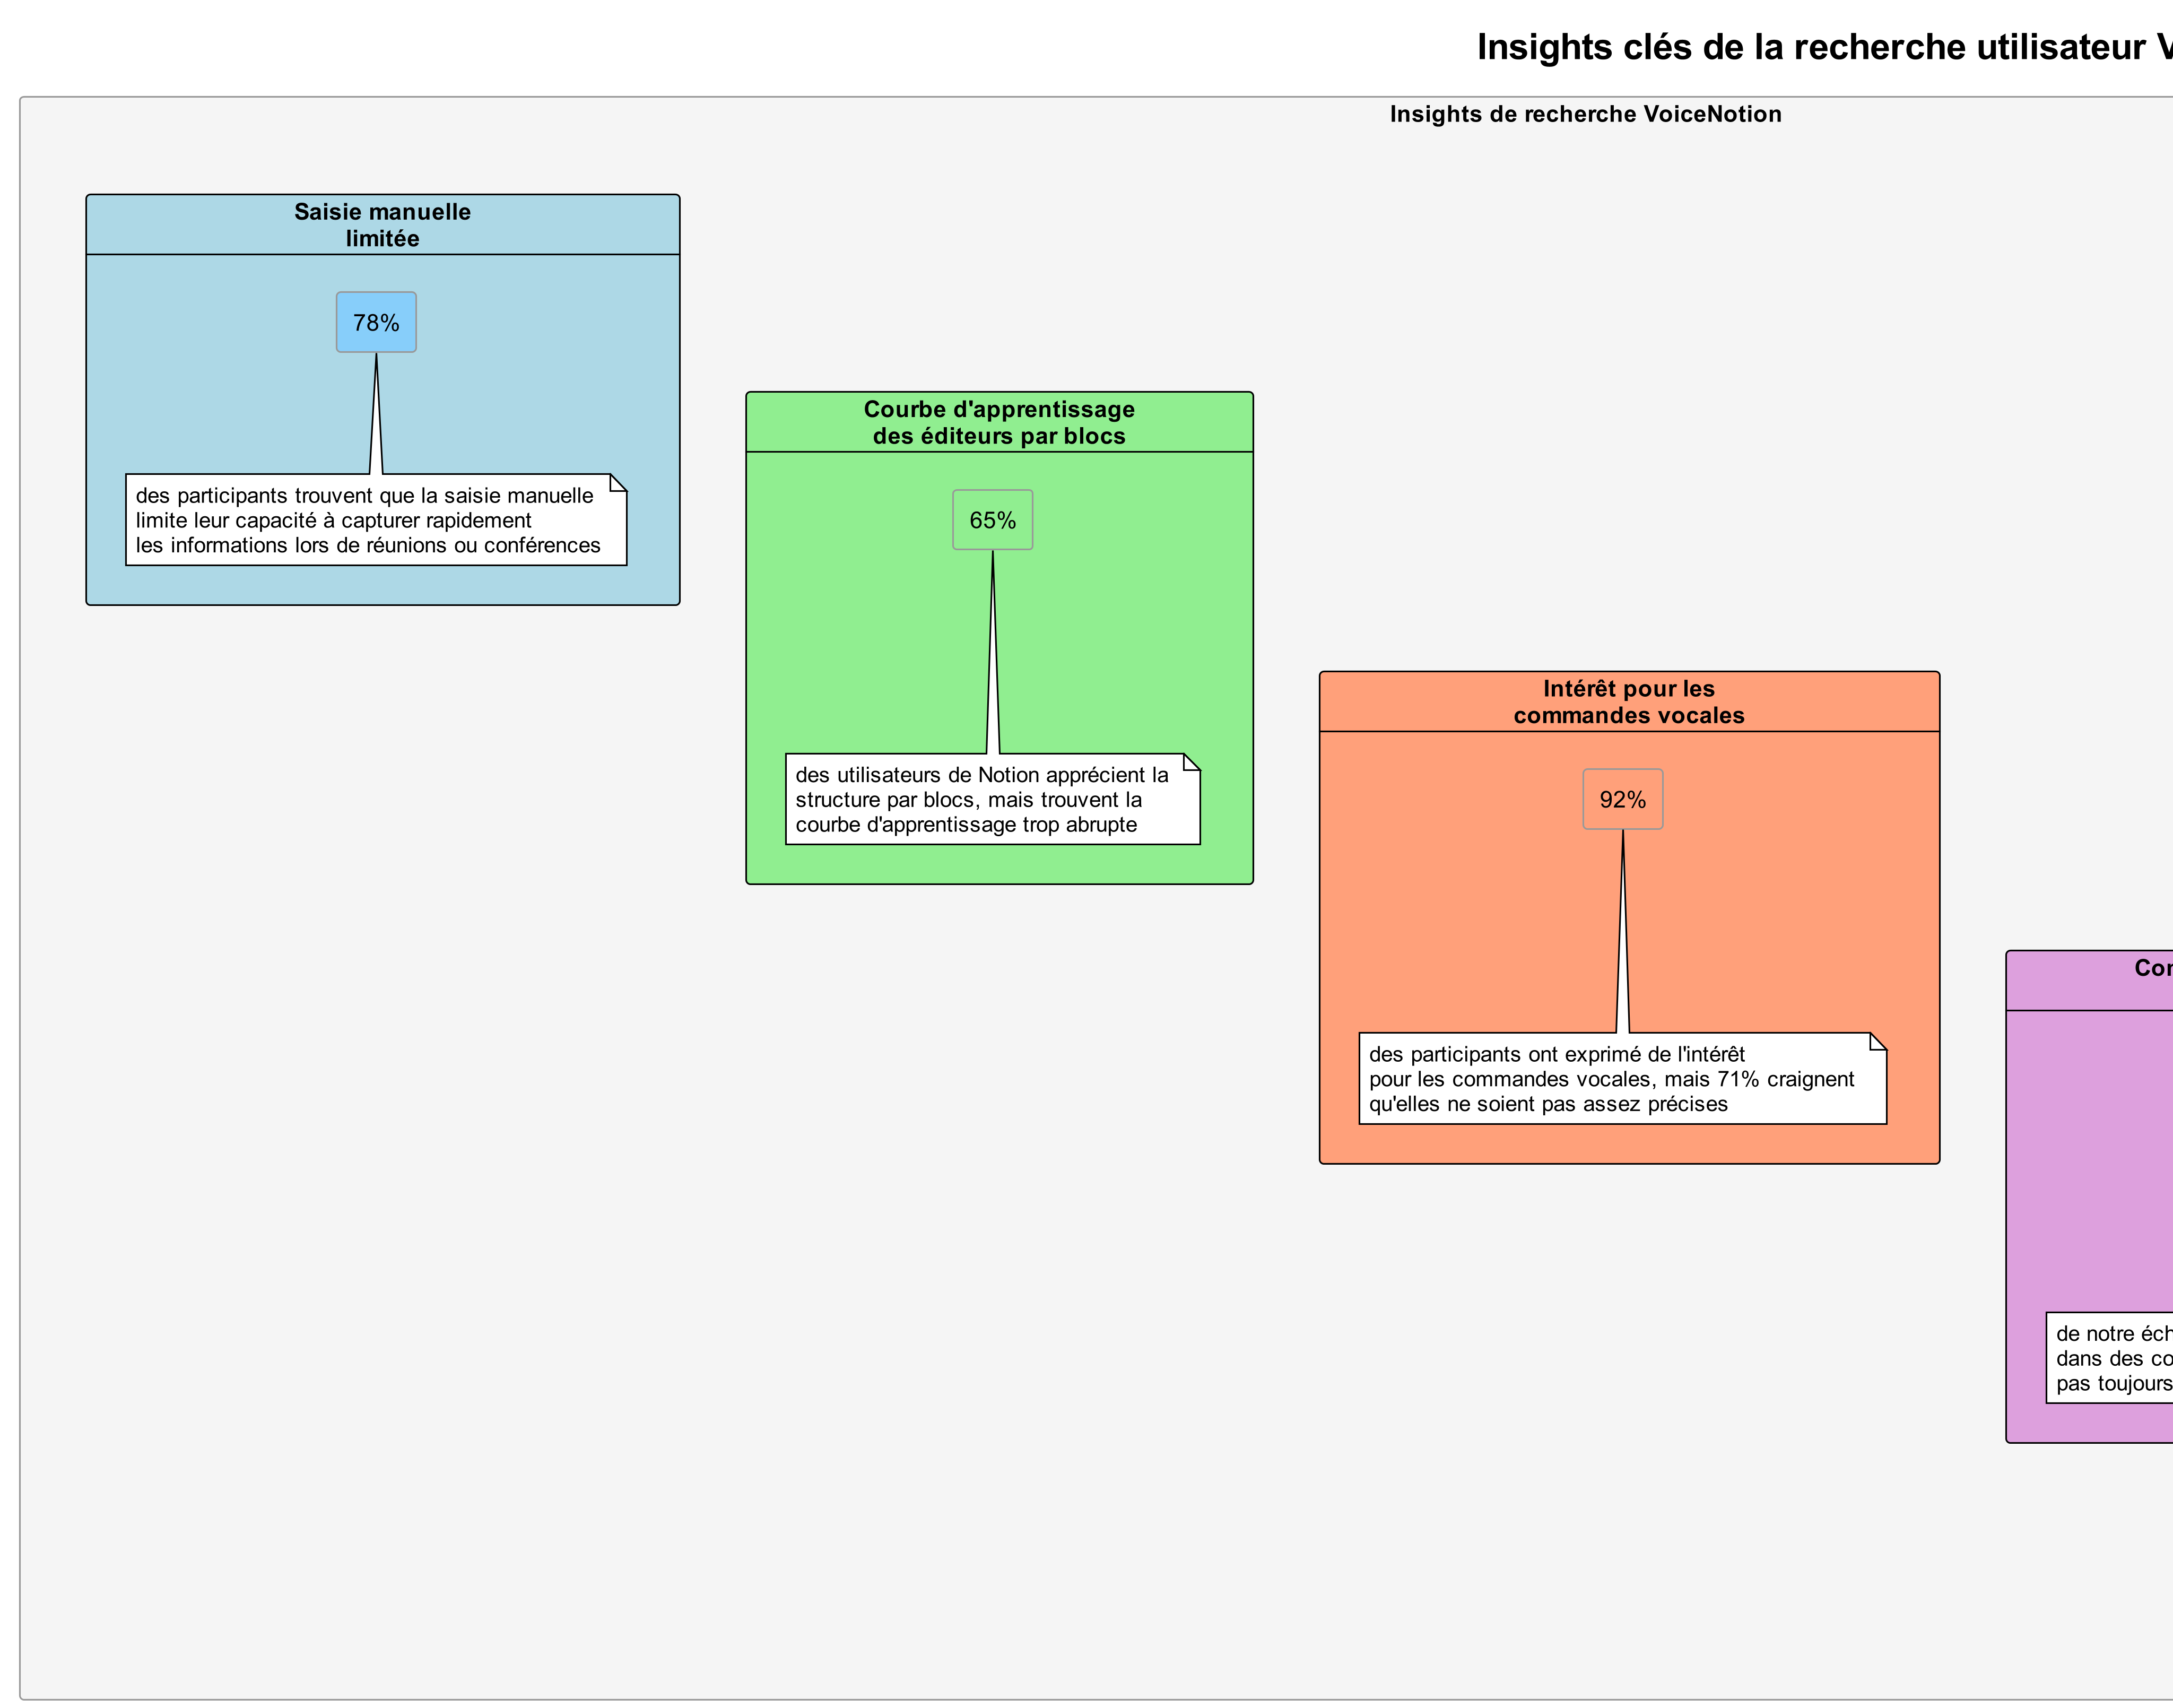
\includegraphics[width=0.75\textwidth]{assets/docs/user_research_insights.png}
    \caption{Synthèse des principaux insights de recherche utilisateur}
    \label{fig:user_research_insights}
\end{figure}

\subsection{Empathie}

\subsubsection{Personas utilisateur}

Basés sur notre recherche, nous avons développé trois personas principaux qui représentent nos utilisateurs cibles:

\paragraph{Persona 1: Sophie l'Étudiante}

\begin{itemize}
    \item \textbf{Profil:} 22 ans, étudiante en master de droit, utilise principalement son smartphone et son ordinateur portable pour prendre des notes.
    \item \textbf{Objectifs:} Capturer efficacement les informations en cours, organiser ses révisions, créer des liens entre différents concepts juridiques.
    \item \textbf{Frustrations:} Difficulté à suivre le rythme des professeurs, perd du temps à reformater ses notes, trouve la navigation entre ses documents fastidieuse.
    \item \textbf{Comportements:} Prend des notes pendant les cours, les complète en bibliothèque, révise régulièrement avec des mind maps et des fiches synthétiques.
    \item \textbf{Citation:} "Je passe plus de temps à essayer de noter tout ce que dit le prof qu'à vraiment comprendre le cours."
\end{itemize}

\paragraph{Persona 2: Marc le Professionnel}

\begin{itemize}
    \item \textbf{Profil:} 38 ans, chef de projet dans une entreprise technologique, toujours en déplacement entre réunions et sites clients.
    \item \textbf{Objectifs:} Capturer rapidement les décisions et actions des réunions, organiser ses projets, partager les informations avec son équipe.
    \item \textbf{Frustrations:} Manque de temps pour prendre des notes détaillées, difficultés à capturer des idées en déplacement, oublie des détails importants.
    \item \textbf{Comportements:} Utilise son téléphone pour des notes rapides, son ordinateur portable pour des documents plus structurés, souvent en multitâche.
    \item \textbf{Citation:} "Entre deux réunions, je n'ai parfois que 5 minutes pour noter les points clés avant d'enchaîner."
\end{itemize}

\paragraph{Persona 3: Leila la Créatrice de Contenu}

\begin{itemize}
    \item \textbf{Profil:} 29 ans, auteure et créatrice de contenu indépendante, travaille depuis chez elle ou dans des cafés.
    \item \textbf{Objectifs:} Capturer l'inspiration quand elle survient, structurer ses idées en articles ou en scripts, organiser ses recherches.
    \item \textbf{Frustrations:} Perd ses meilleures idées quand elle ne peut pas les noter immédiatement, passe trop de temps à organiser son contenu, lutte avec différents formats de notes.
    \item \textbf{Comportements:} Alterne entre notes vocales, notes manuscrites et documents numériques, travaille de manière non linéaire avec beaucoup d'itérations.
    \item \textbf{Citation:} "Mes meilleures idées me viennent souvent quand je suis loin de mon ordinateur, pendant une promenade ou sous la douche."
\end{itemize}

\begin{figure}[H]
    \centering
    %\includegraphics[width=0.9\textwidth]{assets/docs/voicenotion_personas.png}
    \caption{Les trois personas principaux de VoiceNotion}
    \label{fig:voicenotion_personas}
\end{figure}

\subsubsection{Scénarios d'utilisations}

Pour chaque persona, nous avons développé des scénarios d'utilisation qui illustrent comment VoiceNotion répondrait à leurs besoins spécifiques:

\paragraph{Scénario 1: Sophie en cours de droit constitutionnel}

Sophie assiste à un cours de droit constitutionnel où le professeur parle rapidement et fait référence à de nombreux articles et précédents. Avec VoiceNotion, elle:
\begin{enumerate}
    \item Active l'application et commence à prendre des notes textuelles de base.
    \item Utilise la commande vocale "Nouveau titre: Articles constitutionnels importants" pour créer une section structurée sans interrompre sa prise de notes.
    \item Dit "Ajouter liste à puces" pour commencer une liste des articles mentionnés.
    \item Alterne facilement entre la saisie vocale pour les concepts généraux et la saisie manuelle pour les termes techniques précis ou les références.
    \item À la fin du cours, utilise la commande "Créer une sous-page pour les cas jurisprudentiels" pour organiser les exemples mentionnés dans une structure hiérarchique.
\end{enumerate}

\paragraph{Scénario 2: Marc en réunion client puis en déplacement}

Marc participe à une réunion importante avec un client pour discuter des spécifications d'un nouveau projet:
\begin{enumerate}
    \item Au début de la réunion, il ouvre VoiceNotion et crée une nouvelle note avec la structure de base (objectifs, spécifications, actions).
    \item Pendant la discussion, il ajoute rapidement des points à chaque section avec des commandes vocales discrètes.
    \item Il utilise la commande "Ajouter liste à puces: Points à suivre" pour créer une liste d'actions à réaliser.
    \item Après la réunion, dans le taxi, il révise ses notes et utilise la commande vocale "Réorganiser: déplacer la section Budget après Échéancier" pour restructurer son document.
    \item Il crée une sous-page pour les détails techniques qui nécessitent une exploration plus approfondie.
\end{enumerate}

\paragraph{Scénario 3: Leila trouve l'inspiration pendant une promenade}

Leila fait une promenade quotidienne quand elle a une idée pour un nouvel article:
\begin{enumerate}
    \item Elle sort son téléphone et ouvre VoiceNotion, puis dit "Nouvelle note: Idée d'article sur la créativité et la routine".
    \item En marchant, elle dicte ses idées principales, utilisant des commandes comme "Nouveau paragraphe" ou "Point important" pour structurer sa pensée.
    \item Elle dit "Ajouter référence: livre Flow de Mihaly Csikszentmihalyi" pour ne pas oublier cette source.
    \item De retour chez elle, elle reprend la note sur son ordinateur, où elle peut voir la structure déjà organisée et commencer à développer chaque section.
    \item Elle utilise la fonctionnalité de bloc toggle pour cacher certaines sections et se concentrer sur l'introduction qu'elle rédige maintenant manuellement.
\end{enumerate}

\section{Conception du système d'information}

\subsection{Identification des acteurs}

Le système VoiceNotion interagit avec plusieurs types d'acteurs, chacun ayant des objectifs et des interactions spécifiques:

\begin{itemize}
    \item \textbf{Utilisateur non authentifié:} Peut explorer la landing page, créer un compte ou se connecter.
    
    \item \textbf{Utilisateur authentifié:} Le principal acteur du système, qui peut créer, modifier, organiser et exporter des notes.
    
    \item \textbf{API Gemini:} Acteur système externe qui traite les commandes vocales et retourne des instructions structurées.
    
    \item \textbf{Service de stockage:} Acteur système responsable de la persistance et de la synchronisation des données.
\end{itemize}

\subsection{Diagramme de cas d'utilisation}

Le diagramme de cas d'utilisation ci-dessous illustre les principales interactions entre les acteurs et le système VoiceNotion:

\begin{figure}[H]
    \centering
    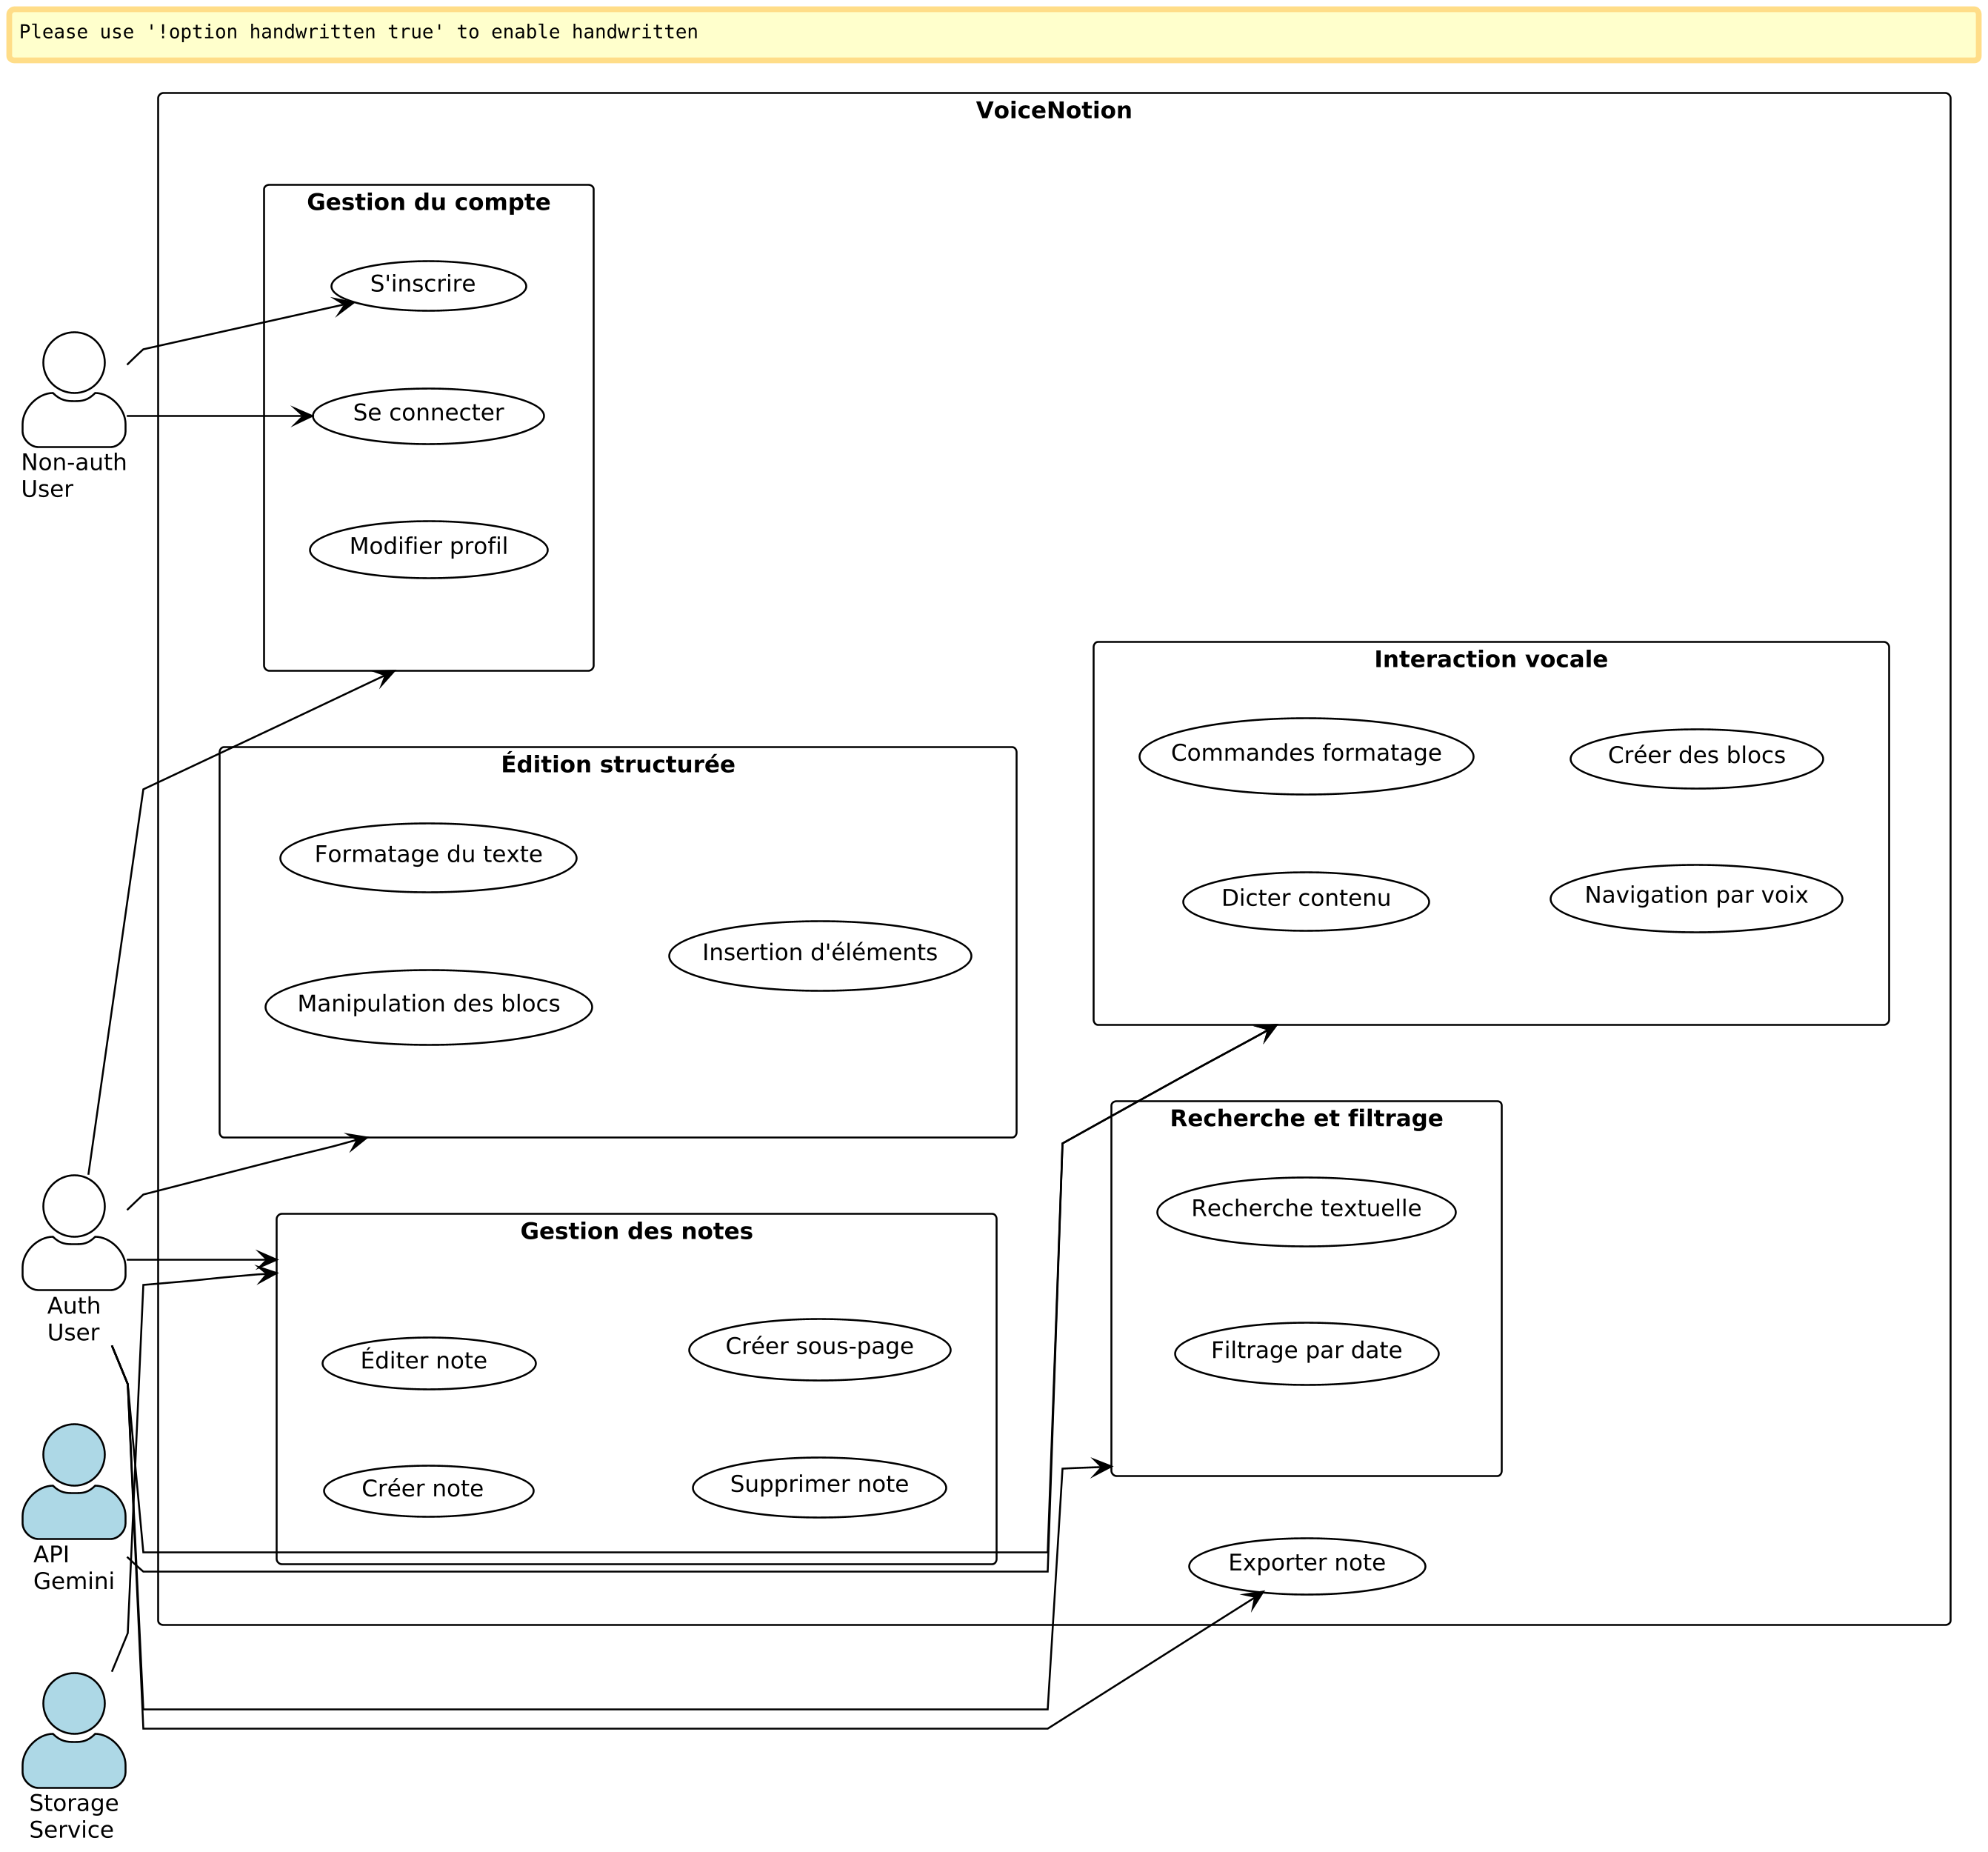
\includegraphics[width=0.9\textwidth]{assets/docs/voicenotion_use_case.png}
    \caption{Diagramme de cas d'utilisation pour VoiceNotion}
    \label{fig:use_case_diagram}
\end{figure}

Les principaux cas d'utilisation incluent:

\begin{itemize}
    \item \textbf{Gestion du compte:} Inscription, connexion, modification du profil.
    
    \item \textbf{Gestion des notes:} Création, édition, suppression, création de sous-pages.
    
    \item \textbf{Interaction vocale:} Dictée de contenu, commandes de formatage, navigation par la voix.
    
    \item \textbf{Édition structurée:} Manipulation des blocs, formatage du texte, insertion d'éléments riches.
    
    \item \textbf{Recherche et filtrage:} Recherche textuelle, filtrage par date.
    
    \item \textbf{Exportation:} Export des notes vers différents formats.
\end{itemize}

\subsection{Diagrammes de séquence}

Pour illustrer les interactions dynamiques entre l'utilisateur, l'application et les services externes, nous avons créé des diagrammes de séquence pour les processus clés.

\subsubsection{Séquence de commande vocale}

Le diagramme suivant montre la séquence d'interactions lors de l'utilisation d'une commande vocale pour manipuler le contenu:

\begin{figure}[H]
    \centering
    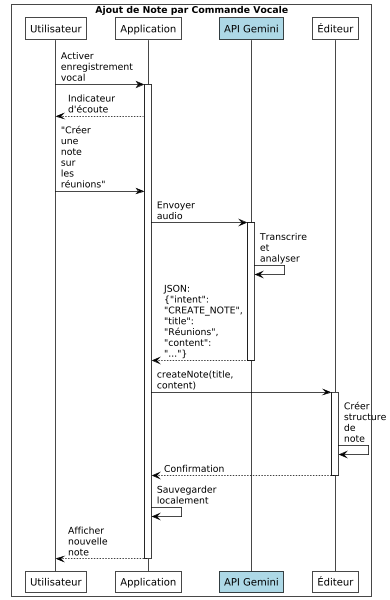
\includegraphics[width=0.85\textwidth]{assets/docs/voicenotion_sequence_voice.png}
    \caption{Diagramme de séquence pour le traitement d'une commande vocale}
    \label{fig:sequence_voice_command}
\end{figure}

\subsubsection{Séquence de création et sauvegarde de note}

Ce diagramme illustre le processus de création, d'édition et de sauvegarde d'une note:

\begin{figure}[H]
    \centering
    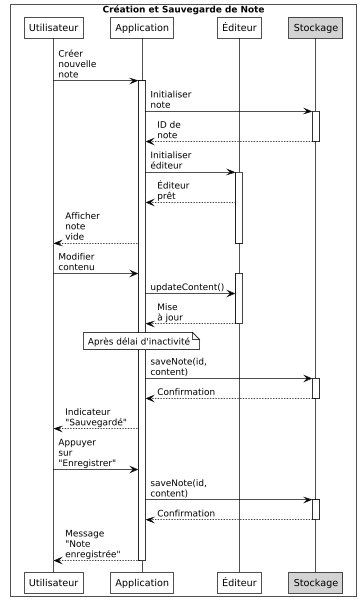
\includegraphics[width=0.85\textwidth]{assets/docs/voicenotion_sequence_save.png}
    \caption{Diagramme de séquence pour la création et sauvegarde d'une note}
    \label{fig:sequence_save_note}
\end{figure}

\subsubsection{Séquence d'authentification}

Ce diagramme illustre le processus d'authentification des utilisateurs dans l'application:

\begin{figure}[H]
    \centering
    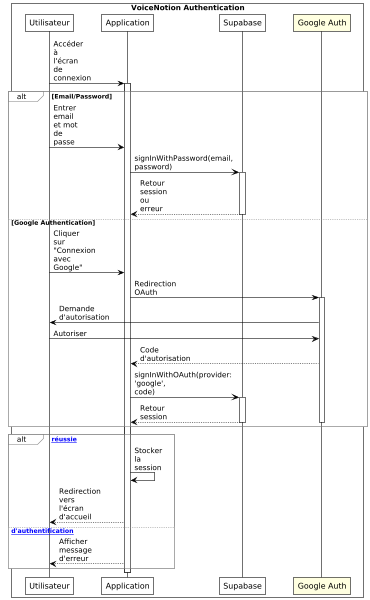
\includegraphics[width=0.85\textwidth]{assets/docs/voicenotion_auth_sequence.png}
    \caption{Diagramme de séquence pour l'authentification}
    \label{fig:sequence_auth}
\end{figure}

\subsection{Diagrammes de base de données}

\subsubsection{Diagramme entité-relation}

Le modèle entité-relation ci-dessous représente la structure conceptuelle des données pour VoiceNotion:

\begin{figure}[H]
    \centering
    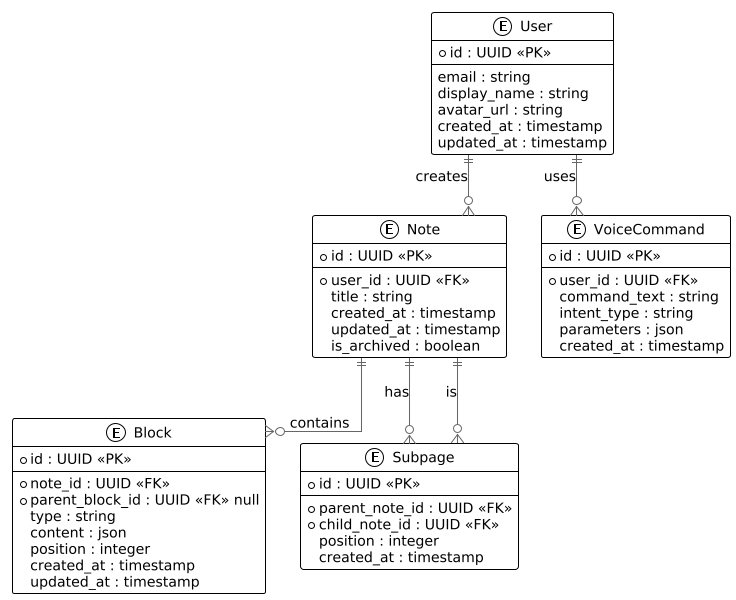
\includegraphics[width=0.9\textwidth]{assets/docs/voicenotion_er_diagram.png}
    \caption{Diagramme entité-relation pour VoiceNotion}
    \label{fig:er_diagram}
\end{figure}

Les principales entités et leurs relations sont:

\begin{itemize}
    \item \textbf{User:} Stocke les informations utilisateur (email, nom d'affichage, avatar).
    
    \item \textbf{Note:} L'entité centrale qui contient les métadonnées d'une note (titre, date de création/modification, propriétaire).
    
    \item \textbf{Block:} Représente un bloc individuel dans une note, avec son type, contenu et position.
    
    \item \textbf{Subpage:} Gère la relation hiérarchique entre les notes, permettant la création de sous-pages.
    
    \item \textbf{VoiceCommand:} Stocke les commandes vocales et leurs paramètres.
\end{itemize}

\subsubsection{Diagramme de base de données}

Le schéma logique de la base de données traduit le modèle entité-relation en une structure implémentable:

\begin{figure}[H]
    \centering
    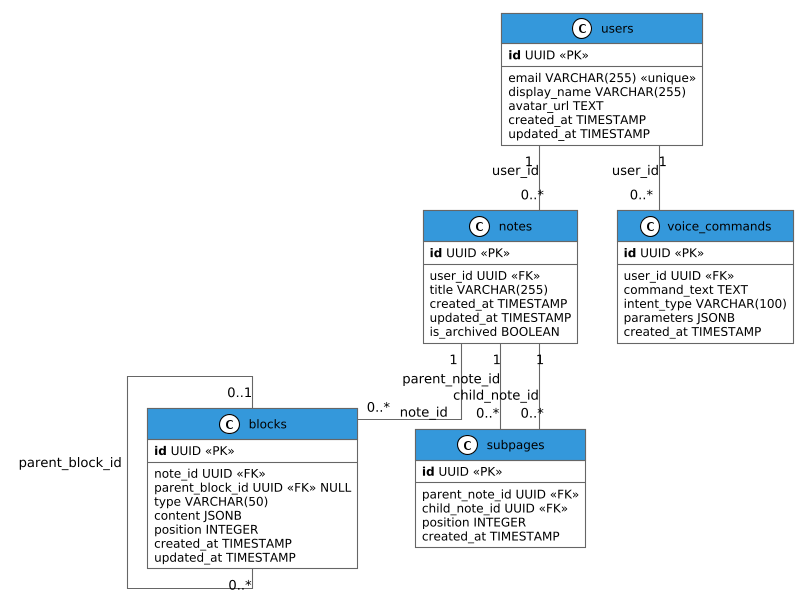
\includegraphics[width=0.9\textwidth]{assets/docs/voicenotion_db_schema.png}
    \caption{Schéma logique de la base de données pour VoiceNotion}
    \label{fig:db_schema}
\end{figure}

Notre implémentation utilise une base de données PostgreSQL hébergée sur Supabase, avec les tables principales suivantes:

\begin{itemize}
    \item \textbf{users:} id, email, display\_name, avatar\_url, created\_at, updated\_at
    
    \item \textbf{notes:} id, title, user\_id, created\_at, updated\_at, is\_archived
    
    \item \textbf{blocks:} id, note\_id, parent\_block\_id, type, content, position, created\_at, updated\_at
    
    \item \textbf{subpages:} id, parent\_note\_id, child\_note\_id, position, created\_at
    
    \item \textbf{voice\_commands:} id, user\_id, command\_text, intent\_type, parameters, created\_at
\end{itemize}

\section{Conclusion}

Ce chapitre a présenté notre approche méthodique de la planification du projet VoiceNotion et de la conception de son expérience utilisateur. En combinant une méthodologie agile avec une approche de Design Thinking centrée sur l'utilisateur, nous avons établi un cadre solide pour le développement d'une application qui répond véritablement aux besoins des utilisateurs.

La recherche utilisateur approfondie et l'élaboration de personas détaillés nous ont permis de comprendre intimement les défis et les aspirations de nos utilisateurs cibles. Les scénarios d'utilisation ont illustré comment VoiceNotion s'intégrerait naturellement dans leurs flux de travail quotidiens, offrant une valeur réelle et des améliorations tangibles à leur expérience de prise de notes.

La conception technique du système, illustrée par les diagrammes de cas d'utilisation, de séquence et de base de données, fournit une base solide pour l'implémentation qui sera détaillée dans le chapitre suivant. Cette architecture a été conçue pour être robuste, évolutive et flexible, permettant d'accommoder les futures améliorations et extensions de l'application.

Les prochaines étapes consistent à transformer cette conception en un produit fonctionnel à travers le développement technique, en restant fidèle à notre vision d'une application de prise de notes révolutionnaire qui libère la créativité et la productivité de ses utilisateurs grâce à la puissance de la voix. 
